\documentclass[11pt, letterpaper, includehead]{article}

%%%%%%%%%%%%%%%%%%%%% Pre-document %%%%%%%%%%%%%%%%%%%%%
\usepackage{fancyhdr}  % Allow for headers
\usepackage{graphicx}  % Allow for figures 
\usepackage{float}     % Allow for figure inserted in specified location
\usepackage{array}     % Allow for cell width manipulation
\usepackage{nicematrix}
\usepackage{multicol} % Multiple cols
\usepackage{tikz} % For latex graphics

\setlength{\parindent}{0pt} % Remove auto paragraph indents

% Get rid of those big ass margins
\usepackage[margin=1in]{geometry}

% Table cell formatting
\setlength{\arrayrulewidth}{0.25mm}
\setlength{\tabcolsep}{11pt}
\renewcommand{\arraystretch}{1.2}

\begin{document}

%%%%%%%%%%%%%%%%%%%%% Title Page %%%%%%%%%%%%%%%%%%%%%
\begin{titlepage}
  \begin{center}
    \Huge{\textbf{Lab 5}}\\
    \Huge{Forces and Acceleration}
    \vfill
    \begin{figure}[H] % H makes the figure insert at the position in the document
      \centering
      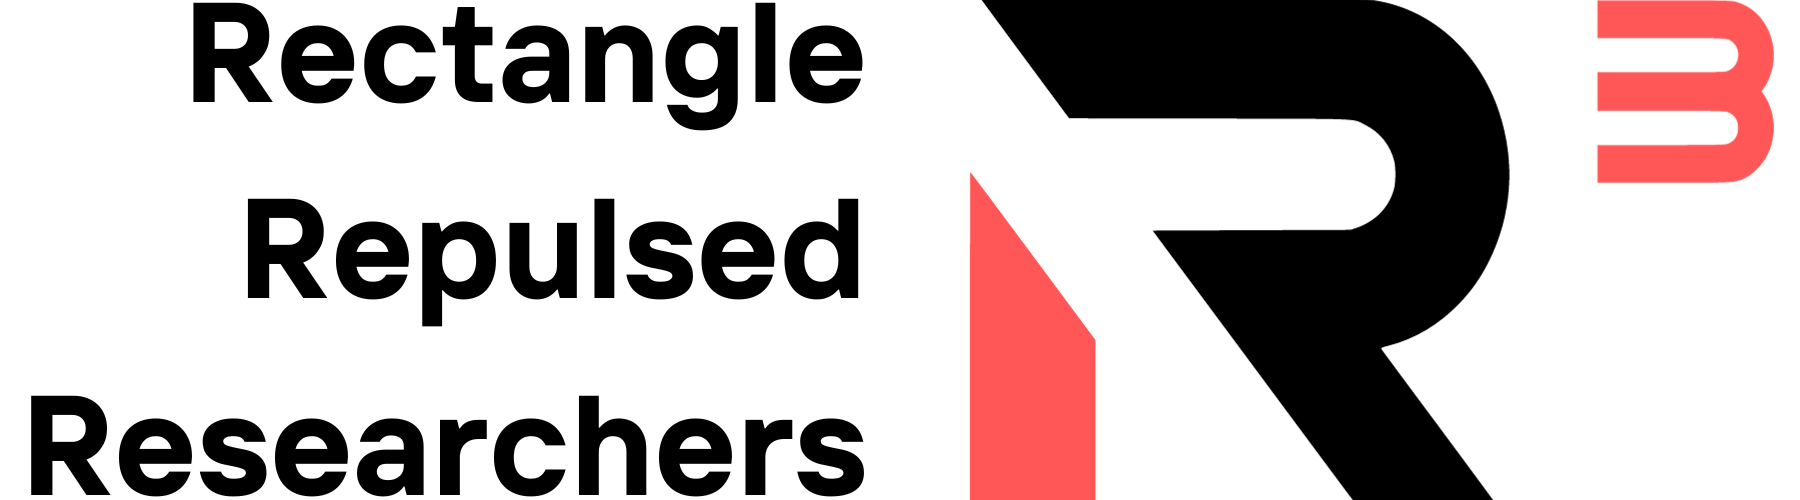
\includegraphics[width=6cm]{../logo.png}
    \end{figure}
    \large{\textbf{your name here}}\\
    \large{Julian Barossi, Liam Gilligan, Stephanie L'Heureux}\\
    \vspace{0.5cm}
    \normalsize
    \today
  \end{center}
\end{titlepage}

%%%%%%%%%%%%%%%%%%%%% TABLE OF CONTENTS %%%%%%%%%%%%%%%%%%%%%
\tableofcontents
\pagebreak % Move to next page

% Add a nice fancy header
\pagestyle{fancy}
\fancyhead{}
\fancyhead[C]{\textbf{Lab 5:} Forces and Acceleration}

%%%%%%%%%%%%%%%%%%%%%%%% SECTION 1 %%%%%%%%%%%%%%%%%%%%%%%%
\section{Level track} % 1
\begin{multicols}{2}
  \centering
  \begin{tikzpicture}
    \draw[thin,dashed][->] (-2,0) -- (2,0) node[right] {$x$}; % x axis
    \draw[thin,dashed][<-] (0,-2) node[below] {$y$} -- (0,2); % y axis
    \draw[very thick, blue][->]  (0,0) --  node [right, pos=1, color=black] {$T$} (0,1); % tension
    \draw[very thick, blue][->]  (0,0) -- node [right, pos=1, color=black] {$m_1g$} (0,-1.5); % weight
    \draw[fill=black] (0,0) circle (0.08); % point in the center
  \end{tikzpicture}

  \columnbreak

  \begin{tikzpicture}
    \draw[thin,dashed][->] (-2,0) -- (2,0) node[right] {$x$}; % x axis
    \draw[thin,dashed][->] (0,-2) -- (0,2) node[above] {$y$}; % y axis
    \draw[very thick, blue][->]  (0,0) --  node [right, pos=1, color=black] {$n$} (0,1); % normal
    \draw[very thick, blue][->]  (0,0) -- node [right, pos=1, color=black] {$m_2g$} (0,-1); % weight
    \draw[very thick, blue][->]  (0,0) -- node [below, pos=1, color=black] {$T$} (1.5, 0); % tension
    \draw[fill=black] (0,0) circle (0.08); % point in the center
  \end{tikzpicture}
\end{multicols}

\subsection{Predicted acceleration of the system} % 1.2
\subsubsection{Solve tensions}
\begin{multicols}{2}
  \centering\textbf{Mass 1}
  $$\sum F = m_1 a$$
  $$m_1 g - T = m_1 a$$

  \columnbreak

  \centering\textbf{Mass 2}
  $$\sum F = m_2 a$$
  $$T = m_2a$$
\end{multicols}

\subsubsection{System acceleration}
$$m_1 g - T = m_1 a$$
$$m_1 g - m_2 a = m_1 a$$
$$m_1 a + m_2 a = m_1 g$$
$$a(m_1 + m_2) = m_1 g$$
$$a = \frac{m_1 g}{m_1 + m_2}$$
$$a = \frac{0.005kg \cdot 9.8m/s^2}{0.005kg + 0.149kg}$$
$$a = \frac{7}{22}m/s^2 \approx 0.32 m/s^2$$
$$\boxed{a =  0.32 m/s^2}$$

\subsection{Predicted time} % 1.3
$$\Delta x = v_ot + \frac{1}{2}at^2$$
$$\Delta x = (0m/s)t + \frac{1}{2}at^2$$
$$\Delta x = \frac{1}{2}at^2$$
$$t = \sqrt{\frac{2\Delta x}{a}}$$
$$t = \sqrt{\frac{2 \cdot 0.908 m}{\frac{7}{22}m/s^2}}$$
$$t = 2.389022514...s \approx 2.39s$$
$$\boxed{t = 2.39s}$$

\subsection{Experimental time}
\begin{center}
  \begin{tabular}{|  m{5cm} | m{5cm} | }
    \hline
    \textbf{Trial}        & \textbf{Time (s)} \\
    \hline
    1                     & 2.24              \\
    \hline
    2                     & 2.34              \\
    \hline
    3                     & 2.41              \\
    \hline
    4                     & 2.29              \\
    \hline
    5                     & 2.37              \\
    \hline
    6                     & 2.32              \\
    \hline
    7                     & 2.42              \\
    \hline
    8                     & 2.25              \\
    \hline
    9                     & 2.30              \\
    \hline
    10                    & 2.40              \\
    \hline
    \hline
    \boldmath{$t_{expt}$} & 2.33              \\
    \hline
    \boldmath{$\sigma_t$} & 0.07              \\
    \hline
    \boldmath{$SE$}       & 0.02              \\
    \hline
  \end{tabular}
\end{center}

\subsection{Analysis} % 1.5
$$t_{expt} \pm 2SE$$
$$2.334s \pm 2( 0.020558858593479 s)$$
$$2.334s \pm 0.04111771718696 s$$
$$t_{thy}\in [2.34788 s, 2.43012 s]$$
$$2.389 \in [2.34788 s, 2.43012 s]$$
The data is consistent with the experiment, $t_{thy}$ falls within two standard errors of $t_{exp}$.

\subsection{Tension} % 1.6
$$T = m_2 \left( \frac{m_1 g}{m_1 + m_2} \right)$$
$$T = 0.149kg \left( \frac{0.005kg \cdot 9.8m/s^2}{0.005kg + 0.149kg} \right)$$
$$T = 0.468285714...N \approx 0.47N $$
$$\boxed{T = 0.47N}$$

%%%%%%%%%%%%%%%%%%%%%%%% SECTION 2 %%%%%%%%%%%%%%%%%%%%%%%%
\section{Sloping air track I} % 2
\subsection{Free body diagram}
\begin{multicols}{2}
  \centering
  \begin{tikzpicture}
    \draw[thin,dashed][->] (-2,-2) -- (2,2) node[right] {$y$}; % x axis
    \draw[thin,dashed][->] (-2,2) -- (2,-2) node[right] {$x$}; % x axis
    \draw[very thick, blue][->]  (0,0) --  node [below, pos=1, color=black] {$mg$} (0,-2); % weight
    \draw[very thick, blue][->]  (0,0) --  node [right, pos=1, color=black] {$n$} (1,1); % normal
    \draw[fill=black] (0,0) circle (0.08); % point in the center
  \end{tikzpicture}

  \columnbreak

  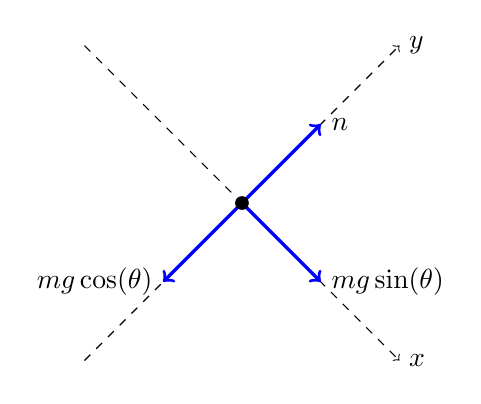
\begin{tikzpicture}
    \draw[thin,dashed][->] (-2,-2) -- (2,2) node[right] {$y$}; % x axis
    \draw[thin,dashed][->] (-2,2) -- (2,-2) node[right] {$x$}; % x axis
    \draw[very thick, blue][->]  (0,0) --  node [left, pos=1, color=black] {$mg\cos(\theta)$} (-1,-1); % weight y
    \draw[very thick, blue][->]  (0,0) --  node [right, pos=1, color=black] {$mg\sin(\theta)$} (1,-1); % weight y
    \draw[very thick, blue][->]  (0,0) --  node [right, pos=1, color=black] {$n$} (1,1); % normal
    \draw[fill=black] (0,0) circle (0.08); % point in the center
  \end{tikzpicture}
\end{multicols}


\subsection{Predicted acceleration of the system}

\subsubsection{Calculate theta}
\begin{multicols}{2}
  $$\theta = \arcsin\left(\frac{0.054m}{0.986m}\right)$$
  $$\theta = 2.61582757013583...^{\circ} \approx 2.62^{\circ}$$
  $$\boxed{\theta = 2.62^{\circ}}$$

  \columnbreak

  \begin{center}
    \begin{tabular}{|  m{3cm} | m{1cm} | m{1cm} | }
      \hline
      \textbf{Quantity} & \boldmath{$cm$} & \boldmath{$m$} \\
      \hline
      Block height      & 4.50            & 0.054          \\
      \hline
      Track length      & 98.60           & 0.986          \\
      \hline
      \hline
      \boldmath{$\theta$} \textbf{(degrees)} & \multicolumn{2}{l|}{2.62} \\
      \hline
    \end{tabular}
  \end{center}
\end{multicols}

\hspace*{0.5cm}

\subsubsection{System acceleration}
$$\sum F_x = ma$$
$$mg\sin(\theta) = ma$$
$$a = g\sin(\theta)$$
$$a = 9.8m/s\sin(2.616^{\circ})$$
$$a = 0.447291125...m/s^2 \approx 0.45m/s^2$$
$$\boxed{a = 0.45m/s^2}$$

\subsection{Predicted time}
$$\Delta x = v_ot + \frac{1}{2}at^2$$
$$\Delta x = (0m/s)t + \frac{1}{2}at^2$$
$$\Delta x = \frac{1}{2}at^2$$
$$t = \sqrt{\frac{2\Delta x}{a}}$$
$$t = \sqrt{\frac{2 \cdot 1.382 m}{0.44729m/s^2}}$$
$$t = 2.485847171...s \approx 2.49s$$
$$\boxed{t = 2.49s}$$

\subsection{Experimental time}
\begin{center}
  \begin{tabular}{|  m{5cm} | m{5cm} | }
    \hline
    \textbf{Trial}        & \textbf{Time (s)} \\
    \hline
    1                     & 2.24              \\
    \hline
    2                     & 2.24              \\
    \hline
    3                     & 2.27              \\
    \hline
    4                     & 2.26              \\
    \hline
    5                     & 2.19              \\
    \hline
    6                     & 2.24              \\
    \hline
    7                     & 2.18              \\
    \hline
    8                     & 2.21              \\
    \hline
    9                     & 2.29              \\
    \hline
    10                    & 2.26              \\
    \hline
    \hline
    \boldmath{$t_{expt}$} & 2.24              \\
    \hline
    \boldmath{$\sigma_t$} & 0.04              \\
    \hline
    \boldmath{$SE$}       & 0.01              \\
    \hline
  \end{tabular}
\end{center}

\subsection{Analysis}
$$t_{expt} \pm 2SE$$
$$2.238s \pm 2( 0.01113552872566 s)$$
$$2.238s \pm 0.0222710574513 s$$
$$t_{thy}\in [2.21573s, 2.26027s]$$
$$2.486s \notin [2.21573s, 2.26027s]$$
The data is not consistent with the experiment, $t_{thy}$ does not fall within two standard errors of $t_{exp}$.

%%%%%%%%%%%%%%%%%%%%%%%% SECTION 3 %%%%%%%%%%%%%%%%%%%%%%%%
\section{Sloping air track II} % 3
\subsection{Free body diagram}
\begin{multicols}{3}

  \centering
  \begin{tikzpicture}
    \draw[thin,dashed][->] (-2,0) -- (2,0) node[right] {$x$}; % x axis
    \draw[thin,dashed][<-] (0,-2) node[below] {$y$} -- (0,2); % y axis
    \draw[very thick, blue][->]  (0,0) --  node [right, pos=1, color=black] {$T$} (0,1); % tension
    \draw[very thick, blue][->]  (0,0) -- node [right, pos=1, color=black] {$m_1g$} (0,-1.5); % weight
    \draw[fill=black] (0,0) circle (0.08); % point in the center
  \end{tikzpicture}

  \columnbreak

  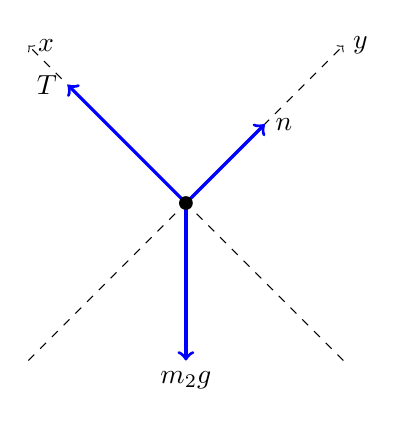
\begin{tikzpicture}
    \draw[thin,dashed][->] (-2,-2) -- (2,2) node[right] {$y$}; % x axis
    \draw[thin,dashed][->] (2,-2) -- (-2,2) node[right] {$x$}; % x axis
    \draw[very thick, blue][->]  (0,0) --  node [below, pos=1, color=black] {$m_2g$} (0,-2); % weight
    \draw[very thick, blue][->]  (0,0) --  node [right, pos=1, color=black] {$n$} (1,1); % normal
    \draw[very thick, blue][->]  (0,0) --  node [left, pos=1, color=black] {$T$} (-1.5,1.5); % tension
    \draw[fill=black] (0,0) circle (0.08); % point in the center
  \end{tikzpicture}

  \columnbreak

  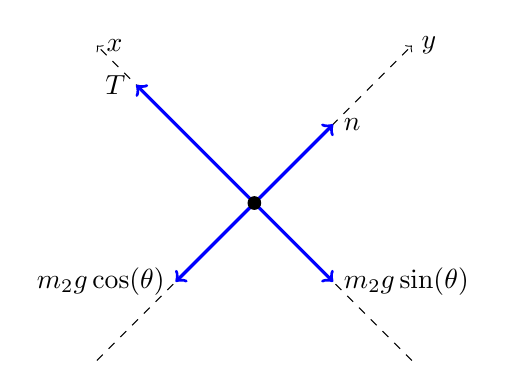
\begin{tikzpicture}
    \draw[thin,dashed][->] (-2,-2) -- (2,2) node[right] {$y$}; % x axis
    \draw[thin,dashed][->] (2,-2) -- (-2,2) node[right] {$x$}; % x axis
    \draw[very thick, blue][->]  (0,0) --  node [left, pos=1, color=black] {$m_2g\cos(\theta)$} (-1,-1); % weight y
    \draw[very thick, blue][->]  (0,0) --  node [right, pos=1, color=black] {$m_2g\sin(\theta)$} (1,-1); % weight y
    \draw[very thick, blue][->]  (0,0) --  node [right, pos=1, color=black] {$n$} (1,1); % normal
    \draw[very thick, blue][->]  (0,0) --  node [left, pos=1, color=black] {$T$} (-1.5,1.5); % normal
    \draw[fill=black] (0,0) circle (0.08); % point in the center
  \end{tikzpicture}
\end{multicols}

\subsection{Predicted acceleration of the system}
\subsubsection{Calculate theta}
\begin{multicols}{2}
  $$\theta = \arcsin\left(\frac{0.054m}{0.986m}\right)$$
  $$\theta = 2.61582757013583...^{\circ} \approx 2.62^{\circ}$$
  $$\boxed{\theta = 2.62^{\circ}}$$

  \columnbreak

  \begin{center}
    \begin{tabular}{|  m{3cm} | m{1cm} | m{1cm} | }
      \hline
      \textbf{Quantity} & \boldmath{$cm$} & \boldmath{$m$} \\
      \hline
      Block height      & 4.50            & 0.054          \\
      \hline
      Track length      & 98.60           & 0.986          \\
      \hline
      \hline
      \boldmath{$\theta$} \textbf{(degrees)} & \multicolumn{2}{l|}{2.62} \\
      \hline
    \end{tabular}
  \end{center}
\end{multicols}

\hspace*{0.5cm}

\subsubsection{Solve tensions}
\begin{multicols}{2}
  \centering\textbf{Mass 1}
  $$\sum F = m_1 a$$
  $$m_1 g - T = m_1 a$$
  $$m_1 g - m_1 a = T$$

  \columnbreak

  \centering\textbf{Mass 2}
  $$\sum F = m_2 a$$
  $$T - m_2 g \sin(\theta) = m_2 a$$
  $$T = m_2 g \sin(\theta) + m_2 a$$
\end{multicols}

\hspace*{0.5cm}

\subsubsection{System acceleration}
$$m_1 g - m_1 a = m_2 g \sin(\theta) + m_2 a$$
$$m_1 g - m_2 g \sin(\theta) = m_2 a + m_1 a$$
$$m_1 g - m_2 g \sin(\theta) = a(m_1 + m_2)$$
$$a = \frac{m_1 g - m_2 g \sin(\theta)}{m_1 + m_2}$$
$$a = \frac{g(m_1  - m_2  \sin(\theta))}{m_1 + m_2}$$
$$a = \frac{(9.8m/s^2)(0.015 kg - 0.149kg \sin(2.616^{\circ}))}{0.015 kg + 0.149kg}$$
$$a = 0.489961112...m/s^2 \approx 0.49m/s^2$$
$$\boxed{a = 0.49m/s^2}$$

\subsection{Predicted time}
$$\Delta x = v_ot + \frac{1}{2}at^2$$
$$\Delta x = (0m/s)t + \frac{1}{2}at^2$$
$$\Delta x = \frac{1}{2}at^2$$
$$t = \sqrt{\frac{2\Delta x}{a}}$$
$$t = \sqrt{\frac{2 \cdot 0.908 m}{0.490m/s^2}}$$
$$t = 1.925129203...s \approx 1.93s$$
$$\boxed{t = 1.93s}$$

\subsection{Experimental time}
\begin{center}
  \begin{tabular}{|  m{5cm} | m{5cm} | }
    \hline
    \textbf{Trial}        & \textbf{Time (s)} \\
    \hline
    1                     & 1.88              \\
    \hline
    2                     & 1.88              \\
    \hline
    3                     & 1.92              \\
    \hline
    4                     & 2.06              \\
    \hline
    5                     & 1.97              \\
    \hline
    6                     & 1.85              \\
    \hline
    7                     & 1.93              \\
    \hline
    8                     & 1.91              \\
    \hline
    9                     & 2.03              \\
    \hline
    10                    & 2.01              \\
    \hline
    \hline
    \boldmath{$t_{expt}$} & 1.94              \\
    \hline
    \boldmath{$\sigma_t$} & 0.07              \\
    \hline
    \boldmath{$SE$}       & 0.02              \\
    \hline
  \end{tabular}
\end{center}

\subsection{Analysis}
$$t_{expt} \pm 2SE$$
$$1.944s \pm 2( 0.0223208920570443 s)$$
$$1.944s \pm 044641784114089 s$$
$$t_{thy}\in [1.89936s, 1.98864s]$$
$$1.93\in [1.89936s, 1.98864s]$$
The data is consistent with the experiment, $t_{thy}$ falls within two standard errors of $t_{exp}$.

\subsection{Tension}
$$T = m_1 \left(g - \frac{g(m_1  - m_2  \sin(\theta))}{m_1 + m_2}\right)$$
$$T = 0.015 kg \left(9.8m/s^2 - \frac{(9.8m/s^2)(0.015 kg - 0.149kg \sin(2.616^{\circ}))}{0.015 kg + 0.149kg}\right)$$
$$T = 0.139651...N \approx 0.14N$$
$$\boxed{T = 0.14N}$$

\end{document}
